\newpage
\section{Experiments}

A comprehensive evaluation has been conducted of this method and a set of robust baselines, employing Convolutional Neural Networks (ConvNets), on tasks sourced from the DeepMind Control Suite (DMControl) and a collection of robotic manipulation tasks. DMControl provides a range of challenging and diverse continuous control tasks and is widely recognized as a benchmark for image-based RL. In order to assess the generalization capabilities of our method and the baselines, we subject them to rigorous distribution shifts from the \textbf{DMControl Generalization Benchmark} (DMControl-GB), the \textbf{Distracting Control Suite} (DistractingCS), as well as distribution shifts specific to the robotic manipulation environment. Our evaluation encompasses the analysis of \textit{sample efficiency}, \textit{asymptotic performance}, and \textit{generalization performance} of the methods across these varied scenarios.


\newpage
\subsection{\textbf{Data Augmentation in RL.}}

Figure \ref{fig:data-aug-visualization} provides a comprehensive set of samples for each of the data augmentations considered in this study: 
\begin{itemize}
    \item random \textit{shift}
    \item random convolution (denoted \textit{conv})
    \item random \textit{overlay}
    \item random \textit{cutout}
    \item Gaussian \textit{blur}
    \item random \textit{affine-jitter}
    \item random \textit{rotation}
\end{itemize}
It is emphasized that the random convolution augmentation is not a convolution operation, but rather application of a randomly initialized convolutional layer as in the original proposal.\\
As in previous work  that applies data augmentation to image-based RL, we either clip values or apply a logistic function, whichever is more appropriate, to ensure that output values remain within the $[0, 1)$ interval that unaugmented observations are normalized to. \\
Each of the considered data augmentations are applied to the \textit{walker} and \textit{cartpole} environments and are representative of the \textit{Walker, walk}, \textit{Walker, stand}, \textit{Cartpole, swingup}, and \textit{Cartpole, balance} tasks. To illustrate the diversity of augmentation parameters associated with a given transformation, we provide a total of 6 samples for each data augmentation in each of the two environments. \\

% Previous work applies augmentation to both state $\mathbf{s}^{\textnormal{aug}}_{t} = \tau(\mathbf{s}_{t}, \nu)$ and successor state $\mathbf{s}^{\textnormal{aug}}_{t+1} = \tau(\mathbf{s}_{t+1}, \nu')$ where $\nu,\nu' \sim \mathcal{V}$. 
% The application of weak augmentation, such as random shift, has been shown to improve sample efficiency without causing significant issues. However, it has been observed that strong augmentation, such as random convolution, can lead to instability and poor sample efficiency. The use of stronger and more varied augmentations, including random convolution, random overlay, and affine-jitter, has the potential to enhance generalization to a broader range of Markov Decision Processes (MDPs). Nonetheless, the naive application of wea augmentations has resulted in optimization challenges and reduced sample efficiency.

% We apply random shifts in SVEA and all baselines by default, and aim to stabilize learning under strong augmentation. As such, we refer to observations both with and without the random shift operation as \textit{unaugmented}, and instead refer to observations as \textit{augmented} after application of one of the 6 augmentations considered in our study. 

\begin{figure}[H]
    \centering
    \begin{subfigure}[b]{0.48\textwidth}
        \centering
        
\includegraphics[width=\textwidth]{figures/visualizations/grid_original.png}
        \caption{No augmentation (walker).}
        \vspace{0.1in}
    \end{subfigure}
    \begin{subfigure}[b]{0.48\textwidth}
        \centering
        
\includegraphics[width=\textwidth]{figures/visualizations/grid_cartpole_original.png}
        \caption{No augmentation (cartpole).}
        \vspace{0.1in}
    \end{subfigure}
    \begin{subfigure}[b]{0.48\textwidth}
        \centering
        
\includegraphics[width=\textwidth]{figures/visualizations/grid_shift.png}
        \caption{Random shift (walker).}
        \vspace{0.1in}
    \end{subfigure}
    \begin{subfigure}[b]{0.48\textwidth}
        \centering
        
\includegraphics[width=\textwidth]{figures/visualizations/grid_cartpole_shift.png}
        \caption{Random shift (cartpole).}
        \vspace{0.1in}
    \end{subfigure}
    \begin{subfigure}[b]{0.48\textwidth}
        \centering
        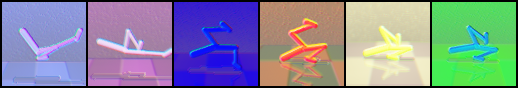
\includegraphics[width=\textwidth]{figures/visualizations/grid_conv.png}
        \caption{Random convolution (walker).}
        \vspace{0.1in}
    \end{subfigure}
    \begin{subfigure}[b]{0.48\textwidth}
        \centering
        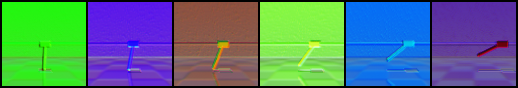
\includegraphics[width=\textwidth]{figures/visualizations/grid_cartpole_conv.png}
        \caption{Random convolution (cartpole).}
        \vspace{0.1in}
    \end{subfigure}
    \begin{subfigure}[b]{0.48\textwidth}
        \centering
        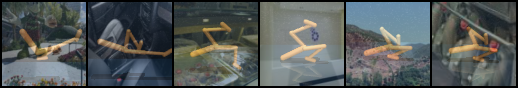
\includegraphics[width=\textwidth]{figures/visualizations/grid_overlay.png}
        \caption{Random overlay (walker).}
        \vspace{0.1in}
    \end{subfigure}
    \begin{subfigure}[b]{0.48\textwidth}
        \centering
        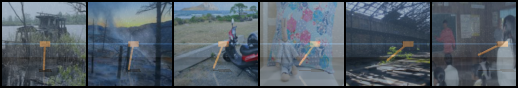
\includegraphics[width=\textwidth]{figures/visualizations/grid_cartpole_overlay.png}
        \caption{Random overlay (cartpole).}
        \vspace{0.1in}
    \end{subfigure}
    \begin{subfigure}[b]{0.48\textwidth}
        \centering
        
\includegraphics[width=\textwidth]{figures/visualizations/grid_cutout.png}
        \caption{Random cutout (walker).}
        \vspace{0.1in}
    \end{subfigure}
    \begin{subfigure}[b]{0.48\textwidth}
        \centering
        
\includegraphics[width=\textwidth]{figures/visualizations/grid_cartpole_cutout.png}
        \caption{Random cutout (cartpole).}
        \vspace{0.1in}
    \end{subfigure}
    \begin{subfigure}[b]{0.48\textwidth}
        \centering
        
\includegraphics[width=\textwidth]{figures/visualizations/grid_blur.png}
        \caption{Random blur (walker).}
        \vspace{0.1in}
    \end{subfigure}
    \begin{subfigure}[b]{0.48\textwidth}
        \centering
        
\includegraphics[width=\textwidth]{figures/visualizations/grid_cartpole_blur.png}
        \caption{Random blur (cartpole).}
        \vspace{0.1in}
    \end{subfigure}
    \begin{subfigure}[b]{0.48\textwidth}
        \centering
        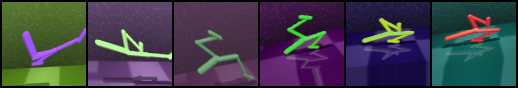
\includegraphics[width=\textwidth]{figures/visualizations/grid_affinejitter.png}
        \caption{Random affine-jitter (walker).}
        \vspace{0.1in}
    \end{subfigure}
    \begin{subfigure}[b]{0.48\textwidth}
        \centering
        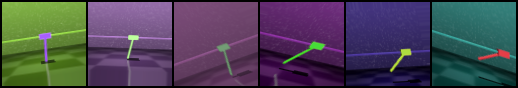
\includegraphics[width=\textwidth]{figures/visualizations/grid_cartpole_affinejitter.png}
        \caption{Random affine-jitter (cartpole).}
        \vspace{0.1in}
    \end{subfigure}
    \begin{subfigure}[b]{0.48\textwidth}
        \centering
        
\includegraphics[width=\textwidth]{figures/visualizations/grid_rotation.png}
        \caption{Random rotation (walker).}
        \vspace{0.1in}
    \end{subfigure}
    \begin{subfigure}[b]{0.48\textwidth}
        \centering
        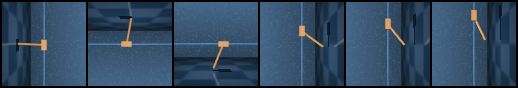
\includegraphics[width=\textwidth]{figures/visualizations/grid_cartpole_rotation.png}
        \caption{Random rotation (cartpole).}
        \vspace{0.1in}
    \end{subfigure}
    \caption{\textbf{Data augmentation}. Visualizations of all data augmentations considered in this study. Left column contains samples from the \textit{Walker, walk} and \textit{Walker, stand} tasks, and right column contains samples from the \textit{Cartpole, swingup} and \textit{Cartpole, balance} tasks.}
    \label{fig:data-aug-visualization}
\end{figure}

The utilization of data augmentation in image-based reinforcement learning (RL) has demonstrated remarkable success by enhancing generalization and regularizing the network parameters of the Q-function and policy $\pi$. However, not all types of augmentations yield equal effectiveness. Studies show that small random crops and random shifts (image translations) significantly enhance the sample efficiency of image-based RL. However, they do not offer significant improvements in generalization to other environments. Conversely, augmentations such as random convolution exhibit substantial potential in improving generalization but are concurrently associated with instability and reduced sample efficiency. In this context, it is crucial to distinguish between \textit{weak} augmentations, such as small random translations, which enhance \textit{sample efficiency} through regularization, and \textit{strong} augmentations, such as random convolution, which improve \textit{generalization} at the cost of sample efficiency. This study specifically focuses on stabilizing deep Q-learning when applying strong data augmentation, aiming to enhance generalization capabilities.

Figure \ref{fig:dmc-svea-augs-generalization} shows training and test performance of SVEA implemented using each of the 6 data augmentations considered in this work. SVEA exhibits comparable stability and sample efficiency for all augmentations, but we find that generalization ability on the \texttt{color\_hard} benchmark of DMControl-GB is highly dependent on the choice of augmentation. Generally, we observe that augmentations such as \textit{conv}, \textit{overlay}, and \textit{affine-jitter} achieve the best generalization, but they empirically also cause the most instability in our \textit{DrQ + aug} baseline as shown in Figure \ref{fig:drq-augs-suppl}.
\begin{figure}[H]
    \centering
    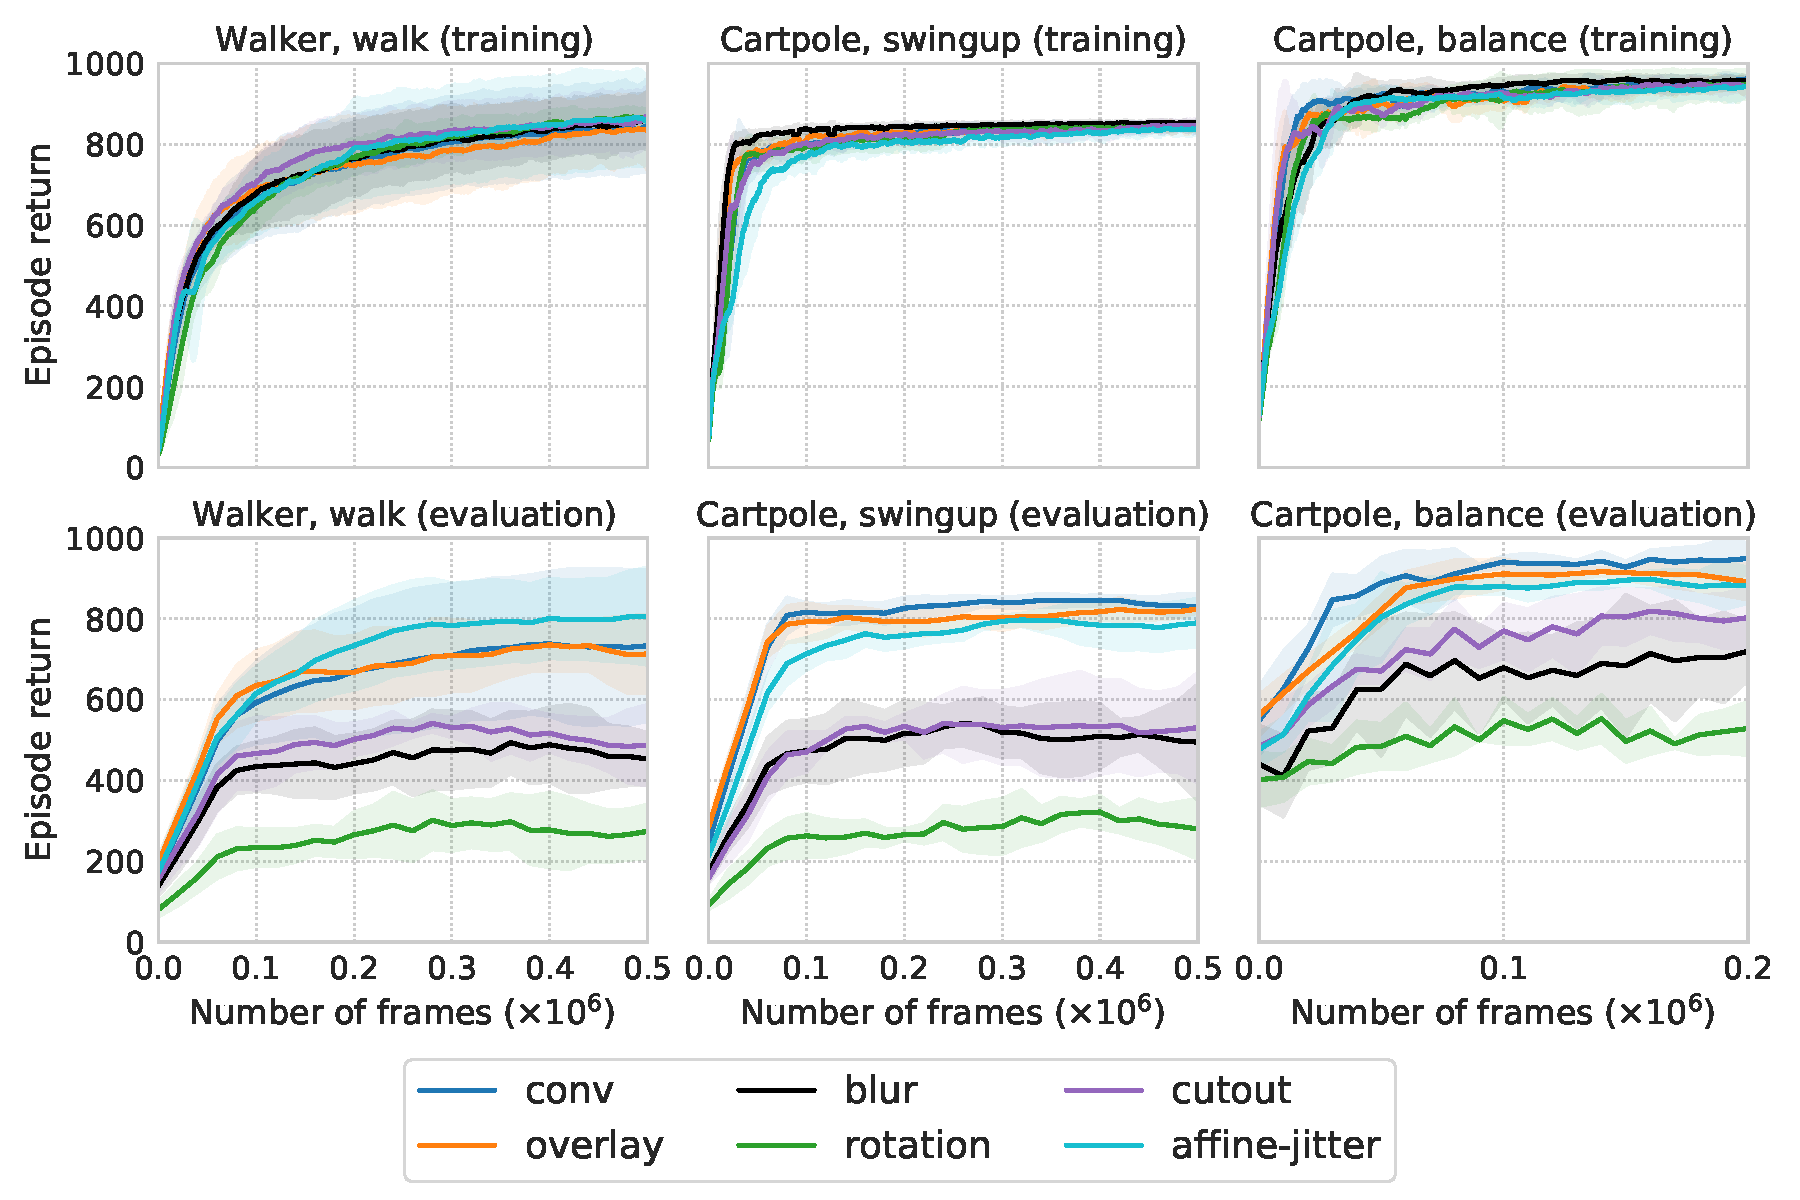
\includegraphics[width=0.64\textwidth]{figures/svea_augs_generalization.pdf}
    \vspace{-0.05in}
    \caption{\textbf{Generalization depends on the choice of data augmentation.} A comparison of SVEA implemented using each of the 6 data augmentations considered in this work (using ConvNets). SVEA exhibits comparable stability and sample efficiency for all augmentations, but generalization ability is highly dependent on the choice of augmentation. \textit{Top:} episode return on the training environment during training. \textit{Bottom:} generalization measured by episode return on the \texttt{color\_hard} benchmark of DMControl-GB. Mean of 5 seeds, shaded area is $\pm1$ std. deviation.}
    \label{fig:dmc-svea-augs-generalization}
    \vspace{-0.1in}
\end{figure}